\documentclass[12pt]{article}
%\usepackage[utf8x]{inputenc}
\usepackage{amsmath}
\usepackage{amssymb}
\usepackage{amsthm}
\usepackage{graphicx}
\usepackage{mathtools}
\usepackage{CJKutf8}

\addtolength{\textwidth}{1.5cm}
\hoffset=-0.7cm
\newcommand{\HH}{\mathcal{H}}
\newcommand{\IP}{\mathbb{P}}
\newcommand{\E}{\mathbb{E}}
\newcommand{\Var}{\mathrm{Var}}
\newcommand{\argmax}{\mathop{\mathrm{arg\,max}}}
\newcommand{\argmin}{\mathop{\mathrm{arg\,min}}}
\newcommand{\eps}{\varepsilon}

\newcommand{\Z}{{\mathbb Z}}
\newcommand{\N}{{\mathbb N}}

\let\phi=\varphi

\newtheorem{theorem}{Theorem}[section]
\newtheorem{corollary}[theorem]{Corollary}
\newtheorem{proposition}[theorem]{Proposition}

\title{The Tangle}
\author{Serguei Popov\thanks{
a.k.a.\ \texttt{mthcl}; 作者聯絡資訊:
\texttt{serguei.popov@iota.org}}
%, for \texttt{Jinn Labs}
}
\date{October 25, 2017. Version 1.4}


\begin{document}
\begin{CJK}{UTF8}{bkai}
 \maketitle
\begin{abstract}  

在本論文中我們分析了 IOTA (一種用於物聯網 [IoT] 行業的加密貨幣) 中所使用的主要技術。
這個新穎的加密貨幣最主要的特點就是 \emph{tangle},以一個有向無環圖 (DAG) 存放交易資訊。
tangle 不僅成功的讓區塊鏈往前邁進一步,其特性更是符合 M2M 小額支付系統的需求。

一個本篇論的關鍵貢獻是馬可夫鏈蒙地卡羅 (Markov Chain Monte Carlo, MCMC) 演算法。
這些演算法會為新的交易選擇要接在哪些既有交易之後。                                        

\end{abstract}

\section{系統介紹與描述}
\label{s_general}

在過去的六年中比特幣的興起和成功證明了區塊鏈技術的價值所在。
然而,這種技術也有許多缺點,阻礙了它成為全球通用的加密貨幣平臺。
在這些缺點中,特別值得提及的就是無法進行小額支付,而小額支付在迅速發展的物聯網行業中的重要性不斷增加。
在現今的系統中,使用者須支付手續費才能產生交易;因此,為了支付極少的金費而須再付好幾倍的手續費並不合理。
且對產生區塊的人而言,手續費就是動機,因此想完全摒除掉並不容易。
另外亦須關注的是現存的加密貨幣都是清楚區分不同角色(如交易發起者,交易驗證者)的異質 (heterogeneous) 系統。
這種明顯區分參與者的設計,容易造成資源搶奪與浪費的現象。
這就需要尋找一些完全不同於比特幣和其他加密貨幣的區塊鏈技術的解決方案。

在本論文中,我們討論了一個創新的方案,但並不能與現今區塊鏈技術相容。
而此方案正以加密貨幣的形式實做,稱之為\emph{IOTA}~\cite{iota},針對物聯網工業所設計。
此篇論文旨在聚焦於 tangle 的一般特性,以及探討當某人試圖捨棄區塊鏈並維護一個分散式帳本時會衍生的問題。
我們並不會討論 iota 具體的實做細節。

在一般情況下,IOTA 按如下方式運行。如前所述,不存在全域的區塊鏈,取而代之的是一個 DAG(有向無環圖),我們稱之為 \emph{Tangle}。
通過節點發出的所有交易構成了這個 Tangle (存所有交易的帳本) 的集合。
這個圖的邊是這樣形成的:當一個新的交易產生,它必須\emph{驗證}之前的兩個\footnote{這是最簡單的方法。
讀者有可能也研讀過相似的系統,規定每筆交易必須驗證 $k$ 筆其他交易,而通常 $k\geq 2$ ,或是採用完全不同的驗證規則。}交易,
這些驗證關係就通過有向的邊來表示,如圖~\ref{f_weights}\footnote{每張圖的時間軸皆為左至右}所示
(在圖中,時間走向皆是從左到右)。
如果從交易~$A$ 到交易~$B$ 之間沒有直接連接的有向邊,而有至少長度為 2 的有向邊路徑存在,我們就說交易~$A$ \emph{間接地驗證}了交易~$B$。
另外,有一個「創世交易」 (genesis trasaction),被所有交易直接或間接驗證,如圖~\ref{f_reverse_weights}。
創世交易的描述如下:在最一開始有一個地址 (address) 擁有全部的 token,接著創世交易會把金錢轉給其他 ``founder'' 的地址。
我們強調所有的 token 皆是創世交易所產生的(不會再產生新的 token),而且不會再有「挖礦」就可以收到金錢獎勵的概念了。\leavevmode\\
術語解釋: \emph{sites}為在 Tangle 圖上的交易;
\emph{節點}(node) 組成整個網路,同時也是交易發起與驗證者。\leavevmode\\
整個架構的宗旨如下:使用者必須驗證其他交易才能發起交易,為整個網路的安全性盡一份力。
我們假設節點檢查認證的交易是否存在衝突。如果節點發現某筆交易與 tangle 的歷史紀錄衝突,便不會直接或者間接的認證具有衝突的交易\footnote{若某節點發起的新交易驗證了衝突交易,
那麼它便有不被其他節點所驗證的風險,而被摒棄。}。
隨著交易被越來越多其他交易直接或者間接的所驗證,這個交易就愈會被系統所接受;
換句話說,要接受一個雙重支付 (double-spending) 交易是極為困難的。
很重要的是我們不會\emph{強制規定}怎麼選擇要驗證的交易;
而是我們認為如果大量的節點依循一些「參考」的規則,
那麼各節點就要分別遵守同類別\footnote{更進一步的論述在~\ref{s_parasite}章節}的規則。這是比較合理的假設,特別是在 IoT,節點是裝載各式韌體的晶片。\leavevmode\\

要發起一個交易,節點需做以下步驟:
\begin{itemize}
  \item 
  根據演算法選擇兩筆交易驗證(這兩筆交易可能會一樣)
  \item 
  檢查這兩筆交易有無衝突,且有皆沒有驗證到衝突的交易
  \item
  要發起一筆合法 (valid) 交易,節點必須解出一道加密的問題,與比特幣相似。
  需要找出一個 nonce 讓其與其他驗證交易的資料的 hash 值為特定格式,如在比特幣的協定中, hash 值得前面需有指定個數個 0
\end{itemize} \leavevmode\\
重要的是, iota 是一個非同步的網路。通常,節點們並不會看到一樣的交易集合。
值得注意的是 tangle 可能存在衝突的交易。
節點間並不需要達成共識,因為合法\footnote{依照協定發起的交易}的交易有權繼續留在帳本中,也就是留在 tangle 中; 
但要是出現衝突的交易,節點便需要決定哪筆交易要被孤立 (orphaned)\footnote{孤立的交易不會再被新進交易間接驗證},也就是這筆交易不會再被新進的交易間接驗證。
決定哪筆交易是要被孤立的主要準則如下: 一個節點進行多次的 tip 選擇演算法\footnote{如上所述,
我們有好的理由可以假設其他節點會遵循一樣的演算法進行 tip 選擇}(cf.\ ~\ref{s_parasite}  節),接著觀察哪筆交易較可能被選到的 tip 間接驗證。
舉例來說: 假設跑了 100 次 tip 選擇演算法,有一筆交易被選到 97 次,我們便說它有 ~$97\%$ 的信心被驗證到。 

我們也一併說明接下來的問題 (cf.\ \cite{red_balloons}): 
促使節點們產生、傳播 (propagate) 交易的動機是什麼? 
每個節點會計算一些數據,其中之一是計算會從鄰居接收多少新的交易。
如果某個特定節點「太懶惰」,便會被它的鄰居捨棄。
因此,即使節點並沒有發起任何的交易,且沒有分享新的交易來驗證自己交易的動力,但他仍然有動機參與。 

在~\ref{s_weight_algo}  節中簡單介紹一些術語後,我們要討論選擇兩筆交易予以接受納入系統的演算法,
用於衡量整體交易的驗證演算法(第~\ref{s_cutsets} 節,尤其是~\ref{s_cum_grow} 節),以及可能會受到的攻擊情況(第~\ref{s_attacks} 節)。 
接著,懼怕數學式的讀者可以直接跳到每一節最後的「結論」。

此外,應該指出的是,有關有向無環圖在加密貨幣領域中的想法已經有一些時日了,
比如文獻 ~\cite{dag_generalized_blockchain, dagcoin, SZ, LSZ, braids}。
尤其需要指出的是,文獻 ~\cite{SZ} 中提出是被稱為 GHOST 的協議,修改了比特幣協議,把主要帳本的結構從區塊鏈改為一棵樹(tree); 
這樣的作法顯示,可以降低驗證時間並提高整體網路的安全性。
在文獻~\cite{LSZ} 中,作者們提出了基於 DAG 的加密貨幣模型; 
有別於我們模型的是,組成 DAG 的是區塊 (block),而非獨立的交易。
且礦工會競爭手續費,新的金錢也會被創造。
再來,文獻~\cite{dagcoin} 中提出了一種類似於我們的解決方案,雖然他並沒有討論任何驗證 tip 的方法。
在這篇論文發布後,也有其他人也研究以 DAG 為基礎的分散式帳本,如~\cite{SZ_SPECTRE}。
我們也提及了另一種~\cite{bitcoinj,lightning} 針對基於 P2P 的比特幣小額支付的解決方案。

\section{Weights and more}
\label{s_weight_algo}
% Here, we define the (own) 
In this section we define the weight of a transaction, 
and related concepts. The weight of a transaction is 
proportional to the amount of work that the issuing node invested 
into it. In 
%practice (meaning ``in current iota's implementation''), 
the current implementation of iota,
the weight may only assume values $3^n$, 
where~$n$ is a positive integer that belongs to 
some nonempty interval of acceptable values\footnote{This
interval should also be finite --- see the ``large weight 
attack'' in Section~\ref{s_attacks}.}.
In fact,
% mostly, here for us 
it is irrelevant to know how the weight
was obtained in practice. 
It is only important that every transaction
has a positive integer, its weight,
% ($=$ weight) 
attached to it. 
 In general, the idea is that a transaction with a
 larger weight is more ``important'' than a transaction
 with a smaller weight.
 % the larger the weight is, the 
% more ``important'' the transaction is for the tangle.
% Usually it is assumed that,
 To avoid spamming and 
 % different kinds of attacks,
 other attack styles, it is assumed that
 no entity can generate
% too many 
an abundance of transactions with ``acceptable'' weights
 in a short period of time.

One of the notions we need is the \emph{cumulative weight}
of a transaction:
it is defined as the own weight of a particular transaction plus
the sum of own weights of all transactions that directly or indirectly approve
this transaction.
The algorithm for cumulative weight calculation is illustrated in 
Figure~\ref{f_weights}. The boxes represent transactions,
the small number in the SE corner of each box denotes own weight, and the 
% (bigger) 
bold number denotes
the cumulative weight. For example, transaction~$F$
is directly or indirectly approved
% , directly or indirectly, 
by transactions
$A,B,C,E$. The cumulative weight of~$F$ is
$9=3+1+3+1+1$, which is the sum of the own weight of~$F$ and the 
own weights of $A,B,C,E$.

 Let us define ``tips'' as unapproved transactions 
 in the tangle graph.
 In the top 
 %picture
 tangle snapshot of 
Figure~\ref{f_weights}, the only 
% unapproved transactions (the ``tips'') 
tips are~$A$ and~$C$.
When the new transaction~$X$ 
% comes 
arrives and approves~$A$ and~$C$ in the bottom 
tangle snapshot,~$X$ becomes the only tip.
 The cumulative weight of all other transactions
increases by~$3$, the own weight of~$X$.
%(which is the weight of~$X$).


\begin{figure}
 \centering 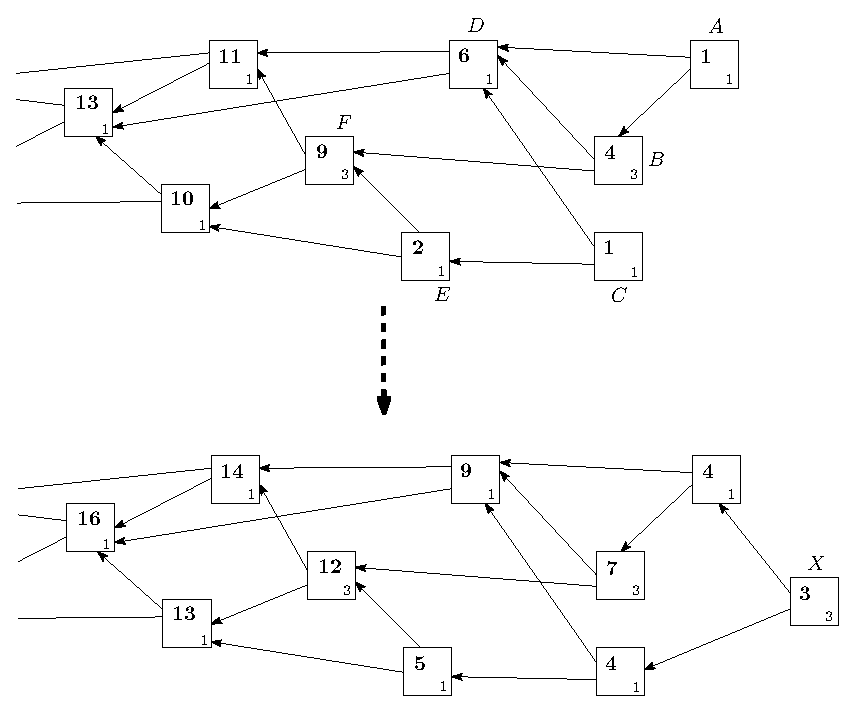
\includegraphics[width=0.64\textwidth]{weights} 
\caption{DAG with weight assignments before and after
a newly issued transaction,~$X$. The boxes represent transactions,
the small number in the SE corner of each box denotes own weight, and the 
bold number denotes the cumulative weight.
%On the weights (re)calculation
}
\label{f_weights}
\end{figure}

% For the discussion of approval algorithms,
We need 
%also 
to introduce two additional variables for the discussion 
of approval algorithms.
First, for a transaction site on the tangle, 
we introduce its
\begin{itemize}
 \item \emph{height}: the length of the longest
oriented path to the genesis;
 \item \emph{depth}: the length of the longest
reverse-oriented path to some tip.
\end{itemize}
For example, 
% on Figure~\ref{f_reverse_weights}, 
$G$ has 
height~$1$ and depth~$4$ 
in Figure~\ref{f_reverse_weights}
% (because of the reverse 
% path $E,C$),
% depth~$3$ 
because of the reverse 
 path $F,D,B,A$, 
while~$D$ has height~$3$ and depth~$2$.
Also, let us introduce the notion of the \emph{score}.
By definition, the score of a transaction
 is the sum of own weights of all transactions approved by this 
transaction plus
 the own weight of the transaction itself.
% (we need this only for the tips, although this definition
% makes sense for all transactions). 
% (again, see 
\begin{figure}
 \centering 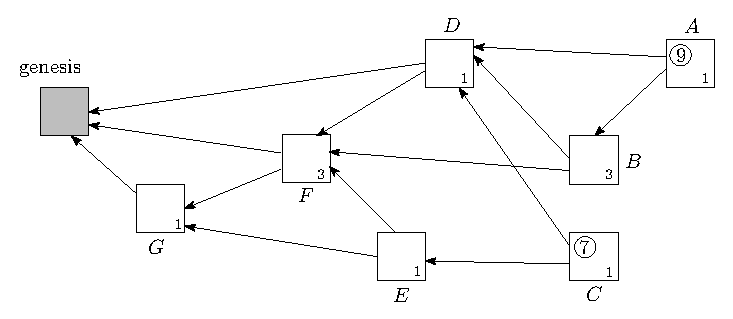
\includegraphics[width=0.64\textwidth]{reverse_weights} 
\caption{
%On the calculation of scores (circled)
DAG with own weights assigned to each site, 
and scores calculated for sites~$A$ and~$C$.}
\label{f_reverse_weights}
\end{figure}
% On the picture, 
In Figure~\ref{f_reverse_weights},
the only 
tips are~$A$ and~$C$.
Transaction~$A$ directly or indirectly approves 
% (directly or indirectly)
transactions $B,D,F,G$, so the score of~$A$
is $1+3+1+3+1=9$. Analogously, the score
of~$C$ is $1+1+1+3+1=7$.

%In fact, 
In order to understand the arguments presented in this paper,
one may safely assume that all transactions have an own weight
 equal to~$1$.  
\emph{From now on, we stick to this assumption}.
% In particular
Under this assumption, the cumulative weight of 
transaction~$X$ becomes
~$1$ plus the number of transactions that directly or 
indirectly approve~$X$, and 
% our transaction directly or indirectly. 
the score 
% now is 
becomes~$1$ plus the number of transactions
that are directly or indirectly approved by~$X$. 
% are directly or indirectly approved by our transaction.

% Also, let us observe that, among the above metrics, 
Let us note that, among those defined 
in this section, the cumulative weight
is (by far!) the most important metric, although 
% for us (although 
height, depth, and score will 
briefly enter some discussions as well.




\section{Stability of the system, and cutsets}
\label{s_cutsets}

Let $L(t)$ be the total number of tips 
% (i.e., unreferenced transactions)
in the system at time~$t$. One
%, of course,
 expects that 
the stochastic process~$L(t)$ remains \emph{stable}\footnote{Under
an additional assumption that the process is time-homogeneous.}.
More precisely, one expects the process to be \emph{positive recurrent}, see Sections~4.4 and~6.5
of~\cite{Ross_m} for formal definitions. 
In particular, positive recurrence implies that the limit of 
$\IP[L(t)=k]$ as $t\to \infty$ should
exist and be positive for all $k\geq 1$. 
Intuitively, we expect that $L(t)$ should fluctuate 
around a constant value, and not escape to infinity.
% (thus leaving a lot of unapproved transactions behind).
If $L(t)$ were to escape to infinity, many unapproved transactions
would be left behind.

To analyze the stability properties of~$L(t)$, we need 
to make some 
assumptions. 
One 
% of them
assumption is that
transactions are issued by a large number
of roughly independent entities, so the process of incoming
transactions can be modeled by a Poisson point process
(cf.\ e.g.\ Section~5.3 of~\cite{Ross_m}).
Let~$\lambda$ be the rate of that Poisson process.
 For simplicity, let us assume 
 %for now 
 that 
this rate remains constant in time. 
Assume that all devices have approximately 
the same computing power, and let~$h$ be the average
time a device needs to perform calculations
that are required to issue a transaction.
% in the case where there are~$L$
% tips and the total number of transactions is~$N$. 
Then, let us \emph{assume} that all nodes
behave in the following way:
 to issue a transaction, a node 
 %just
  chooses
two tips at random and approves them. 
It should be observed that, in general, it is \emph{not}
a good idea for the ``honest nodes'' to adopt
this strategy because it has a number of practical
disadvantages. In particular, it does not offer enough
protection against ``lazy'' or malicious nodes
%\footnote{We 
%remind the reader that we do not try to \emph{enforce}
%any particular tip selection strategy. 
%An attacker can choose tips in any way they find convenient.} 
(see Section~\ref{s_parasite} below). On the other hand,
we still consider this model since it is simple to analyze,
and 
% therefore one may get 
may provide insight into the system's behavior
for more complicated tip selection strategies.
% For this simple strategy, one may assume that the Poisson flows
% of approvals to 
% %different 
% each tip are independent, and have
% rate $2\lambda/L$. This follows from
% Proposition~5.3 of~\cite{Ross_m}, which says 
% that if we independently classify each event of a Poisson process
% according to a list of possible subtypes,
% then the processes of events of each subtype 
% are independent Poisson processes.

Next, we make a further simplifying assumption that any node,
at the moment when it issues a transaction, observes not the 
actual state of the tangle, but the one exactly~$h$ time units
ago. This means, in particular, that a transaction
attached to the tangle at time~$t$ only becomes 
visible to the network at time~$t+h$. We also assume 
that the number of tips remains roughly stationary
in time, and is concentrated around a number~$L_0>0$.
In the following, we will calculate~$L_0$ as
a function of~$\lambda$ and~$h$. 

Observe that,
at a given time~$t$ we have roughly $\lambda h$ ``hidden tips'' 
(which were attached in the time interval $[t-h,t)$ 
 and so are not yet visible to the network);
also, assume that typically there are~$r$ ``revealed tips'' 
 (which were attached before time $t-h$), 
so $L_0 = r+ \lambda h$. 
By stationarity, we may then assume that at time~$t$ there 
are also around~$\lambda h$ sites that were tips at time~$t-h$, 
 but are not tips anymore. 
Now, think about a new transaction that comes at this moment;
then, a transaction it chooses to approve is a tip 
with probability $r/(r+\lambda h)$ (since there are around~$r$
tips known to the node that issued the transaction,
and there are also around~$\lambda h$ transactions which are not 
tips anymore, although that node thinks they are), 
so the mean number of chosen tips is $2r/(r+\lambda h)$. 
The key observation is now that, in the stationary regime,
this mean number of chosen tips should be equal to~$1$,
since, in average, a newcoming transaction should not change
the number of tips.
Solving the equation $2r/(r+\lambda h)=1$ with respect to~$r$, 
we obtain $r=\lambda h$, and so 
\begin{equation}
\label{L0_def} 
L_0 = 2\lambda h.
\end{equation}

We also note that,
if the rule is that a new transaction references~$k$ 
transactions instead of 2, then a similar calculation gives
\begin{equation}
\label{L0k_def} 
 L_0^{(k)} = \frac{k\lambda h}{k-1}.
\end{equation}
This is, of course, consistent with the fact that~$L_0^{(k)}$ 
should tend to $\lambda h$ as $k\to\infty$ (basically, the 
only tips would be those still unknown to the network).



%  Therefore,
% \begin{equation}
% \label{prob_appr_tip}
%  \IP[\text{nobody approves a given tip during time }h(L,N)]
% = \exp\Big(-\frac{2\lambda h(L,N)}{L}\Big).
% \end{equation}
% This means that the expected increment of the total number
% of tips at the moment when our device issues a
% transaction is equal to
% \begin{equation}
% \label{eq_drift}
%  1-2\exp\Big(-\frac{2\lambda h(L,N)}{L}\Big).
% \end{equation}
% In the above formula, ``$1$'' corresponds to the new tip created
% by the transaction, and the second term corresponds to the expected
% number of ``erased'' tips.
% % Indeed, a
% According to~\eqref{prob_appr_tip},
% %(and assuming also that the node always chooses two 
% %\emph{distinct} tips to approve in the event when there
% %are at least two available tips)
%  each tip\footnote{Assuming that the node always chooses two 
% \emph{distinct} tips to approve if there
% are at least two tips available.} that is initially
% chosen for approval will still remain a tip
%  at the moment when the transaction is issued 
% with
% probability~$\exp\big(-\frac{2\lambda h(L,N)}{L}\big)$.
%  Now, $L(t)$ is in fact a continuous-time
% random walk on~$\N=\{1,2,3,\ldots\}$, with nearest-neighbor 
% transitions. 
% %Indeed, i
% If the two chosen transactions were already
% approved, then the process jumps one unit to the right.
% If both chosen transactions were not previously approved, 
% then the process jumps one unit to the left.
%  %and i
%  In the last possible 
% case, the process remains still. 
% 
% %Now, t
% To understand the typical behavior of the process,
% observe that the drift\footnote{The expectation
% of the increment of the number of tips.} 
% %(i.e., the expectation
% %of the increment of the number of tips)
%  in~\eqref{eq_drift} is positive
% for small~$L(t)$ and negative for 
% large~$L$\footnote{This is true for large~$L$
%  in the case when
% $h(L,N)=o(L)$ as $L\to\infty$, or just assuming that 
% the main contribution to the computation or propagation
% time does not come from handling the tips.}. 
% In other words, if~$L(t)$ is small, then the drift has a tendency to
% increase, while if~$L(t)$ is large, the drift has a
% tendency to decrease.
% Therefore, the  ``typical'' 
% value,~$L_0$, of~$L(t)$  
% %be where
% occurs when~\eqref{eq_drift} 
% vanishes so that the number of tips has no 
% clear tendency to increase or decrease. That is, 
% \begin{equation}
% \label{L0_def}
%  L_0 \approx \frac{2\lambda h(L_0,N)}{\ln 2} 
% \approx 2.89\cdot\lambda h(L_0,N).
% \end{equation}

% It is clear that $L_0$, defined above, is the typical size of
% the tip set. 
Also (we return to the case of two transactions to approve) 
the expected time for a transaction to be 
approved for the first time is approximately $h+L_0/2\lambda=2h$.
This is because, by our assumption, during the first~$h$
units of time a transaction cannot be approved, and after
that the Poisson flow
of approvals to it has rate approximately $2\lambda/L_0$. 
(Recall Proposition~5.3 of~\cite{Ross_m}, which says 
that if we independently classify each event of a Poisson process
according to a list of possible subtypes,
then the processes of events of each subtype 
are independent Poisson processes.)

Observe that\footnote{At least in the case where the nodes
\emph{try} to approve tips.} at any fixed time~$t$ the set 
of transactions that were tips
at some moment~$s\in[t,t+h(L_0,N)]$ typically
constitutes a \emph{cutset}. 
% in the sense that 
Any path from 
a transaction issued at time~$t'>t$ to the genesis must pass
through this set. It is important that the size of 
a new cutset in the tangle occasionally becomes small. 
%the cutsets 
%at least occasionally; 
One may then 
use the small cutsets as checkpoints for possible DAG pruning
and other tasks.

% Now, the above ``purely random'' strategy is not 
% very good in practice, 
% because it does not encourage approving tips:
% a ``lazy'' user could just always approve a fixed couple 
% of very old transactions 
% (and therefore not contributing to approval 
% of more recent transactions)
% without being punished for such behavior\footnote{we 
% remind the reader that we do not try to \emph{enforce}
% any particular tip selection strategy, so an 
% attacker can choose tips in any way he/she finds convenient}.
% To discourage the behavior of this sort, one has to adopt a
% strategy which is biased towards the tips with higher score.

It is important to observe
%, however,
 that 
the above ``purely random'' approval 
strategy is not very good in practice 
because it does not encourage approving tips.
A ``lazy'' user could 
%just
always approve a fixed 
%couple 
pair
of very old transactions, therefore not contributing to the approval of 
more recent transactions,
without being punished for such behavior\footnote{We 
remind the reader that we do not try to \emph{enforce}
any particular tip selection strategy. An 
attacker can choose tips in any way they find convenient.}.
Also, a malicious entity can artificially inflate the number
of tips 
%(e.g., 
by issuing many transactions that approve
a fixed pair of transactions. 
%in order to 
This would make it possible for future transactions to
select these tips with very high probability, effectively
 abandoning the tips belonging to ``honest'' nodes.
To avoid issues of this sort, one has to adopt a
strategy that is biased towards the ``better'' tips.
One example of such a strategy is presented in Section~\ref{s_parasite}
below\footnote{The author's feeling is that the tip approval 
strategy is \emph{the} most important ingredient for 
constructing a tangle-based cryptocurrency because 
%It is there that many
attack vectors are hiding in this element of the system.
 Also, since there are usually no ways to 
enforce a particular tip approval strategy, there must be a 
good reason for nodes to voluntarily choose to follow a common 
strategy. A possible reason is knowing that a good portion of other 
nodes are following the same tip approval strategy. 
%that strategy must 
%be such that the nodes would voluntarily choose to follow it
%knowing that at least a good proportion of other nodes does so.
}.


% An example of such a strategy can be the following. 
% Fix a parameter $\alpha\in(0,1)$; 
% then, choose the two transactions to approve between
% the top~$\alpha L$ (with respect to their score).
% The same considerations as above imply that the typical 
% size of the set of tips will be 
% \begin{equation}
% \label{L0alpha_def}
%  L_0^{(\alpha)} \approx \frac{2\lambda h(L_0,N)}{\alpha \ln 2}
%  \approx 2.89\cdot \alpha^{-1}\lambda h(L_0,N).
% \end{equation}
% As for the expected time for a transaction to be 
% approved for the first time, the situation a bit more
% complicated.
Before starting the discussion about 
the expected time for a transaction to 
%be approved for the first time
receive its first approval, 
%observe 
note that
we can distinguish 
%essentially 
two regimes 
(Figure~\ref{f_regimes}).
\begin{itemize}
 \item Low load: the typical number of
tips is small, and frequently becomes~$1$.
This may happen when the flow of transactions is so small
% enough, so
 that it is not probable that several different transactions
approve the same tip. Also, if the network latency is very
low and devices compute fast, it is unlikely
that many tips would appear. This even holds true in the case when the flow
of transactions is reasonably large. Moreover, 
we have to assume that there are no attackers 
that try to artificially inflate the number of tips.
 \item High load: the typical number of tips is large.
This may happen when
the flow of transactions is 
%big enough, 
large, and computational delays together with network
latency make it likely that several different transactions
approve the same tip.
\end{itemize}
\begin{figure}
 \centering 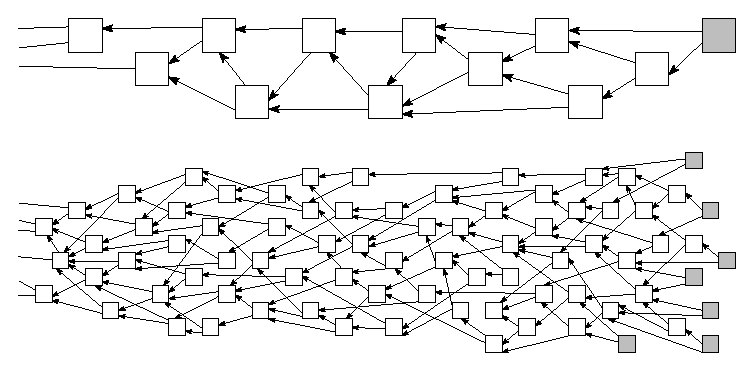
\includegraphics[width=0.64\textwidth]{regimes} 
\caption{Low load (top) and high load (bottom) regimes of 
incoming transaction flow. White squares represent verified 
sites, while gray squares represent tips.
%The tangle and its typical tip sets (shaded) 
%in low load and high load
%regimes. Observe that in the latter case some transactions
%may have to wait a lot until approved for the first time.
}
\label{f_regimes}
\end{figure}
%Of course, t
This division is rather informal, and there is no
clear borderline between the the two regimes. Nevertheless,
we find that it may be instructive to consider these
two 
%essentially 
different 
%situations. 
extremes.

%In the low load regime, the situation is relatively simple:
The situation in the low load regime is relatively simple. The first approval
 happens on an average timescale of order $\lambda^{-1}$
since 
% already the first (or one of the first)
one of the first few 
incoming transactions will approve 
% our transaction.
a given tip.

Let us now consider the high load regime, 
% that is, 
the 
%situation
case where~$L_0$ is large.
As mentioned above, one may assume that
the Poisson flows of approvals to different tips are independent
and have an approximate rate of~$2\lambda/L_0$. Therefore,
 the expected time for a transaction to 
 % be 
% approved for the first time 
receive its first approval is around $L_0/(2\lambda)\approx 1.45 h$
% (recall
~\eqref{L0_def}.
% ).

% First, if the transaction did not make it into
% the top~$\alpha L$, then this waiting time can be quite large,
% of order $\exp(cL_0^{(\alpha)})$ (since there is a drift
% towards $L_0^{(\alpha)}$ for smaller values of~$L$ and the size of the 
% tip set needs to become much smaller than $L_0^{(\alpha)}$ for 
% that transaction to be considered for approval). 
% Therefore, a good strategy
% for the owner of such a transaction would be to issue an additional
% empty transaction referencing the first one, and hope that this
% new transaction enters into the top~$\alpha L$. 
% Also, similarly to the above, if the transaction is one
% of the top~$\alpha L$, then with constant probability
% it will have to wait around $L_0/\lambda$ time units to be
% approved for the first time 
% (observe that $\alpha L_0^{(\alpha)}=L_0$).
% It is worth noting, 
However, 
it is worth noting that for more elaborate
approval strategies\footnote{That favor 
%the tips of the 
``better'' quality tips in future implementations of iota.}, it may not be a good
idea to passively wait a long time until a transaction
is approved by the others. 
%whatever that may mean)
This is 
%because 
due to the fact that ``better'' tips will
keep appearing and will be preferred for approval.
Rather, in the case when a transaction is waiting 
for approval over 
% too long time (i.e., 
a time interval much larger than $L_0/2\lambda$,
a good strategy 
%will
would be 
to promote this latent transaction with an additional empty 
transaction\footnote{An empty transaction is a transaction
that does not involve any token transfer, but still has to
approve two other transactions. It should be noted that 
generating an 
empty transaction contributes 
to the network's security.}. 
% that is, 
In other words, a node can issue an empty transaction that 
approves its previous transaction together with one of the ``better'' tips to 
increase the probability that the empty transaction receives approval.
%so that this empty transaction has a high probability of 
%being approved. 
%good chance to be
%further approved.

% Let us now consider the high load regime.
%  First, if the transaction did not make it into
% the top~$\alpha L$, then this waiting time can be quite large,
% of order $\exp(cL_0^{(\alpha)})$ (since there is a drift
% towards $L_0^{(\alpha)}$ for smaller values of~$L$ and the size of the 
% tip set needs to become much smaller than $L_0^{(\alpha)}$ for 
% that transaction to be considered for approval). 
% Therefore, a good strategy
% for the owner of such a transaction would be to issue an additional
% empty transaction referencing the first one, and hope that this
% new transaction enters into the top~$\alpha L$. 
% Also, similarly to the above, if the transaction is one
% of the top~$\alpha L$, then with constant probability
% it will have to wait around $L_0/\lambda$ time units to be
% approved for the first time 
% (observe that $\alpha L_0^{(\alpha)}=L_0$).
% However, if that did not happen, then the transaction may fall
% below the top~$\alpha L$, and then a good strategy will be 
% to promote it with an additional empty transaction.
% 
% Another easy strategy would be to pick, say,
% five random tips (among all of them), 
% and approve the top two between these five. Again, 
% if your transaction was not approved during time 
% $\Theta(L_0/\lambda)=\Theta(h(L_0,N))$,
% it is a good idea to promote it with an additional empty transaction.
% 
% We also notice that the approval strategy may be further
% modified, for example, to prevent spamming. For example,
%  the nodes might prefer
% tips with bigger own weight, making it more difficult
% for the spammer to have his transactions approved. 

%Now, i
It turns out that the approval strategies based
on heights and scores may be vulnerable to a specific
type of attacks, see Section~\ref{s_parasite}. We will
discuss more elaborate strategies\footnote{In fact, 
the author's feeling is that the tip approval 
strategy is \emph{the} most important ingredient for 
constructing a tangle-based cryptocurrency. It is there that many
attack vectors are hiding. Also, since there is usually no way to 
\emph{enforce} a particular tip approval strategy, it must 
be such that the nodes would voluntarily choose to follow it
knowing that at least a good proportion of other nodes does so.} 
to defend against such attacks
in that section. 
%Nevertheless, 
In the meantime, it is still worth considering
the simple tip selection strategy where an incoming 
transaction approves two random tips. 
%(``approve two random tips''),
This strategy 
%since it 
is the easiest to analyze, and therefore may 
%give 
provide some 
insight into the qualitative and quantitative behavior of the 
%system
tangle.

\paragraph{Conclusions:}
\begin{enumerate}
 \item We distinguish between two regimes, low load and high
load (Figure~\ref{f_regimes}).
 \item There are only a few tips in the low load regime.
 % , usually there are not many tips (say, one or two), and a 
 A
 tip gets approved for the first
time in $\Theta(\lambda^{-1})$ time units, where~$\lambda$ is the rate of the 
incoming flow of transactions.
 \item In the high load regime the typical number 
of tips depends on the tip approval strategy employed by the new 
transaction. 
%(i.e., how the new 
%transaction chooses the other two transactions for approval).
 \item If a transaction uses the strategy of approving two 
 random tips, the typical number of tips is given by~\eqref{L0_def}. 
 % For the ``approve two random tips'' strategy, the 
%typical number of tips is given by
 It can be shown 
that this strategy is optimal with respect to the typical
number of tips. However, it is not practical to adopt this strategy
because it does not encourage approving tips.
%  \item For the strategy ``approve two random tips among top
% $\alpha L(t)$'' (which does not have the above disadvantage), the 
% typical number of tips is given by~\eqref{L0alpha_def}.
 \item More elaborate strategies are needed to handle attacks 
 and other network issues. A family 
 %However, more elaborated strategies are needed; a family
of such strategies 
%will be described 
is discussed in Section~\ref{s_parasite}.
 \item The typical time for a 
 %In the high load regime, the typical time until a
tip to be approved is $\Theta(h)$ in the high load regime, where~$h$ 
is the average computation/propagation time for a node. However, 
if the first approval does not occur in the above time interval,
it is a good idea for the issuer and/or receiver
to promote that transaction with an additional empty transaction.
\end{enumerate}




\subsection{How fast does the cumulative weight typically grow?}
\label{s_cum_grow}

Assume that the network is in the low load regime. 
% Clearly, in the low load regime,
After a transaction gets approved several times, 
its cumulative weight will grow 
with speed~$\lambda$ 
%since essentially
because all new transactions
will indirectly reference this 
transaction\footnote{Recall that we assumed that
the own weights of all transactions are equal to~$1$,
so the cumulative weight is just the number of transactions
that directly or indirectly reference a transaction
plus~$1$.}.

In the case where the network is in the high load regime, an 
old transaction with a large cumulative weight will experience 
weight growth 
%As for the high load regime,
% if a transaction is old enough
%and with big cumulative weight, then the cumulative weight grows
with speed~$\lambda$ 
because essentially 
all new transactions will indirectly reference it.
%for the same reasons.
Moreover, when the transaction is first added to the tangle it may have 
to wait for some time to be approved. In this time interval, the 
transaction's cumulative weight behaves in a random fashion.
% Also, we know
%that in the beginning the transaction may have to wait 
%for some time
%to be approved, and it is clear that its cumulative weight
%behaves in a random fashion at that time.  
% However, observe that during
% a time interval of length~$h(L_0,N)$, in average, a tip 
% will receive $\lambda h(L_0,N)/L_0 \approx \ln 2$ ???
To characterize the speed with which the cumulative weight 
grows after the 
%see how fast the cumulative weight grows after the 
transaction receives several approvals, let us define~$H(t)$
%denote (for simplicity, we start counting time 
%at the moment when our transaction has been created) by
 as the expected cumulative weight at time~$t$ 
(for simplicity, 
we start counting time at the moment when
 our transaction was revealed to the network, i.e.,
$h$ time units after it was created)
 and~$K(t)$ as the expected number of
 tips that approve the transaction at time~$t$.
%(or simply ``our tips'')
Let us also abbreviate $h:=h(L_0,N)$. 
We make a simplifying
assumption that the number of tips remains roughly
constant at a value of~$L_0$ over time. 
%(equal to~$L_0$) in time. 
We work with the ``approve two random tips'' strategy in this section. 
It is expected that the qualitative behavior will be roughly the same for 
other reasonable strategies. 

Recall that a transaction 
%coming to the system 
entering the network at time~$t$ typically 
chooses two 
%transactions 
tips to approve based on the state
of the system at time~$t-h$ because the node must do
some calculations and verifications before actually issuing the 
transaction. 
% Let us make a further simplifying
% assumption that~$h(L_0,N)$ is much less than~$L_0$; essentially
It is not difficult to see that
(assuming, though, that $K(\cdot)$ is the \emph{actual}
number of tips, not just expected number)
%obtain that 
the probability of the transaction approving at least one of ``our'' tips
 in the tangle is
%that it approves at least one``our'' tip is 
$1-\big(1-\frac{K(t-h)}{L_0}\big)^2
=\frac{K(t-h)}{L_0}\big(2-\frac{K(t-h)}{L_0}\big)$\footnote{The expression on the left-hand
 side is~$1$ minus the probability that the two approved tips are not ours.}.
% (indeed, the two approved tips are ours with probability
% $\big(\frac{K(t-h)}{L_0}\big)^2$, ). 
Analogous to Example~6.4 of~\cite{Ross_m},
we can write for small $\delta>0$
\[
 H(t+\delta) = H(t) 
+ \lambda \delta\frac{K(t-h)}{L_0}\Big(2-\frac{K(t-h)}{L_0}\Big)
 + o(\delta),
\]
and thus deduce the following differential equation
\begin{equation}
\label{diff_H}
 \frac{d H(t)}{dt} = \lambda \frac{K(t-h)}{L_0}\Big(2-\frac{K(t-h)}{L_0}\Big).
\end{equation}
In order to be able to use~\eqref{diff_H}, we need to first 
calculate~$K(t)$.
This is not a trivial task since a tip at time~$t-h$ 
may not be a tip at time~$t$, 
and the overall number of tips approving the original transaction 
increases by 1 in the case where an incoming transaction 
approves such a tip.
%It is not immediately clear how to do this, since a tip 
%at time~$t-h$ may not be a tip at time~$t$, and, 
%in the case when the newly coming transaction approves
%such a tip, the overall number of tips approving the original
%transaction increases by~$1$. 
The crucial observation
is that the probability that a tip at time~$t-h$ remains a tip
at time~$t$ is approximately~$1/2$. 
(To verify this, recall the discussion from 
Section~\ref{s_cutsets}: the typical number of tips
is $2\lambda h$, and during the interval of length~$h$
new~$\lambda h$ tips will substitute a half of old ones.)
% plug the expression
%  in~\eqref{L0_def} into~\eqref{prob_appr_tip}.
 Therefore, at time~$t$ approximately one half~$K(t-h)$ 
%``previous'' our 
tips remain in the unconfirmed tip state, while the other half
will have received at least one approval. 
%be already approved at least once. 
Let~$A$ denote
%by~$A$ 
the set of  
%(approximately) 
$K(t-h)/2$ tips at time~$t-h$
that are still tips at time~$t$, and let~$B$ denote the remaining 
set of $K(t-h)/2$ tips that were already approved by time~$t$.
% will be denoted by~$B$. 
Let~$p_1$ be the probability that a new transaction
%the newly arrived transaction 
approves at least~$1$ transaction from~$B$
and does not approve any transactions from~$A$. Furthermore,
let~$p_2$ be the probability that both approved transactions
belong to~$A$. In other words, $p_1$ and~$p_2$ are
the probabilities that the current number of ``our'' tips
increases or decreases by~$1$ upon arrival of the new transaction. 
We have
\begin{align*}
 p_1 &= \Big(\frac{K(t-h)}{2 L_0}\Big)^2 + 2\times
\frac{K(t-h)}{2 L_0}\Big(1-\frac{K(t-h)}{L_0}\Big),  \\
 p_2 &= \Big(\frac{K(t-h)}{2 L_0}\Big)^2.
\end{align*}
To obtain the first expression, observe that~$p_1$
equals the probability that both approved tips 
belong to~$B$ plus twice the probability that the first
tip belongs to~$B$ and the second tip does not 
belong to $A\cup B$.
Analogous to~\eqref{diff_H},
the differential equation for $K(t)$ is:
\begin{equation}
\label{diff_K}
 \frac{d K(t)}{dt} = (p_1-p_2)\lambda = \lambda
 \frac{K(t-h)}{ L_0}\Big(1-\frac{K(t-h)}{L_0}\Big).
\end{equation}
It is difficult to solve~\eqref{diff_K} exactly,
so we make further simplifying assumptions.
First of all, we observe that after the time when~$K(t)$
reaches level~$\eps L_0$ for a fixed~$\eps>0$, it will grow 
very quickly to~$(1-\eps)L_0$. 
%(indeed, the right-hand side of~\eqref{diff_K} will be bounded away from~$0$).
Now, when~$K(t)$ is small with respect to~$L_0$, 
we can drop the last factor in the right-hand side of~\eqref{diff_K}\footnote{It 
would be a constant close to~$1$, so the 
right-hand side would be equivalent to 
$\lambda\frac{K(t-h)}{ L_0}$.}.
% Also, substituting~$K(t-h)$ by $K(t)-h\frac{d K(t)}{dt}$,
% we obtain a simplified version of~\eqref{diff_K}
We obtain a simplified version of~\eqref{diff_K}
by recalling that $\frac{\lambda h}{L_0}=\frac{1}{2}$:
\begin{equation}
\label{diff_K_simpl}
 \frac{d K(t)}{dt} \approx \frac{1}{2h}K(t-h),
%\approx 0.74\cdot \frac{\lambda K(t)}{ L_0},
\end{equation}
with boundary condition $K(0)=1$. 
We look for a solution of the form $K(t)=\exp(c\frac{t}{h})$;
after substituting this into~\eqref{diff_K_simpl},
we obtain
\[
 \frac{c}{h}\exp\Big(c\frac{t}{h}\Big) 
   \approx \frac{1}{2h}\exp\Big(c\frac{t}{h}-c\Big),
\]
therefore 
\begin{equation}
\label{eq_K_simpl}
K(t)=\exp\Big(W\big({\textstyle\frac{1}{2}}\big)\frac{t}{h}\Big)
    \approx \exp\Big(0.352\frac{t}{h}\Big)
\end{equation}
is an approximate solution, where~$W(\cdot)$ is the so-called
Lambert $W$-function.\footnote{Also known as
 the omega function or product logarithm; for~$x\in [0,+\infty)$
it is characterized by the relation $x=W(x)\exp(W(x))$.}
% The 
% (approximate) solution of this differential
% equation is
% \begin{equation}
% \label{eq_K_simpl}
%  K(t) \approx \exp\Big(\frac{t\ln 2}{(2+\ln 2)h}\Big)
% \approx \exp\Big(0.26\frac{t}{h}\Big).
% \end{equation}
Taking the logarithm of both sides in~\eqref{eq_K_simpl}, we find that
the time when~$K(t)$ reaches $\eps L_0$ is roughly
\begin{equation}
 \label{eq_t0}
 t_0 \approx \frac{h}{W\big({\textstyle\frac{1}{2}}\big)} 
\times \big(\ln L_0 - \ln \eps^{-1}\big)
\lesssim 2.84 \cdot h  \ln L_0.
\end{equation}
%Turning back
Returning to~\eqref{diff_H} and 
dropping the last term on the right-hand side, we
obtain that during the ``adaptation period'' (i.e., $t\leq t_0$
with~$t_0$ as in~\eqref{eq_t0}), it holds that
\begin{align*}
 \frac{d H(t)}{dt} &\approx \frac{2\lambda}
{L_0}K(t-h)
  \\
&\approx \frac{1}{h\exp\big(W(\frac{1}{2})\big)}
\exp\Big(W\big({\textstyle\frac{1}{2}}\big)\frac{t}{h}\Big)
\\
&= \frac{2W\big({\textstyle\frac{1}{2}}\big)}{h}
\exp\Big(W\big({\textstyle\frac{1}{2}}\big)\frac{t}{h}\Big)
\end{align*}
and therefore
\begin{equation}
\label{eq_H}
 H(t)\approx 
2\exp\Big(W\big({\textstyle\frac{1}{2}}\big)\frac{t}{h}\Big)
\approx 2\exp\Big(0.352\frac{t}{h}\Big).
\end{equation}

Let us also remind the reader that
% , as discussed above,
 after the adaptation period,
the cumulative weight~$H(t)$ grows linearly
with speed~$\lambda $. We stress that the ``exponential
growth'' in~\eqref{eq_H} does not mean that 
the cumulative weight grows ``very quickly'' 
during the adaptation period. Rather, the behavior
is as depicted in Figure~\ref{f_adapt_period}.
\begin{figure}
 \centering \includegraphics[width=0.64\textwidth]{adapt_period_1} 
\caption{Plot of cumulative weight vs. time for the high load regime.
%On the cumulative weight growth
}
\label{f_adapt_period}
\end{figure}

% Also, we comment that the calculations in this section 
% can be easily adapted to the situation when a node
% references~$s>1$ transactions \emph{in average}. 
% For this, one just need to replace~$2$ by~$s$ in~\eqref{eq_drift}
% (but not in~\eqref{diff_H}!), and $2$ by~$s$ as well as 
% $\ln 2$ by~$\ln s$ in~\eqref{L0_def}
% % --\eqref{L0alpha_def}
% and in \eqref{diff_K_simpl}--\eqref{eq_H}.

\goodbreak

\paragraph{Conclusions:}
\begin{enumerate}
 \item After a transaction gets approved multiple times 
 in the low load regime, 
its cumulative weight will grow 
with speed~$\lambda w$, where~$w$ is the mean weight
of a generic transaction.
 \item In the high load regime, there are two distinct growth 
 phases. First, a transaction's 
% again,after our transaction gets approved several of times,
%first its 
cumulative weight~$H(t)$ grows with increasing
speed during the \emph{adaptation period}
according to~\eqref{eq_H}. After
the adaptation period is over, the cumulative weight grows 
with speed~$\lambda w$ (Figure~\ref{f_adapt_period}).
In fact, for \emph{any} reasonable strategy the cumulative
weight will grow with this speed after the end
of the adaptation period because 
%essentially all newly 
all incoming transactions will indirectly approve  
%our transaction.
the transaction of interest.
 \item One can think of the adaptation period of a 
 transaction as the time until most of the current tips indirectly
approve that transaction. The typical length of the 
adaptation period is given by~\eqref{eq_t0}.
\end{enumerate}


\section{Possible attack scenarios}
\label{s_attacks}
We start by discussing an 
%obvious 
attack scenario where the attacker tries to ``outpace'' the network alone:
% Let us describe an attack scenario:
\begin{enumerate}
 \item An attacker sends a payment to a merchant and receives 
 the goods after the merchant decides the transaction has a sufficiently large
  cumulative weight.
% the attacker pays to the merchant, and receives the 
%goods after the merchant considers that the transaction got already 
%a sufficiently large cumulative weight;
\item The attacker issues a double-spending transaction.
\item \label{x_strategy} The attacker uses their computing
 power to issue many small transactions that approve the
  double-spending transaction, but do not approve the 
  original transaction that they sent to the merchant either 
  directly or indirectly.
%the attacker issues a lot of small transactions
%(very aggressively, with all his computing power)
%that ​do​ ​not​ approve the original 
%one directly or indirectly, but approve the double-spending transaction;
\item It is possible for the attacker to have a plethora of Sybil
 identities which are not required to approve tips.
%observe that the attacker may have a lot of Sybil identities,
%and also is not required to necessarily approve tips;
\item An alternative method to item~\ref{x_strategy}
 would be for the attacker
 to issue a big double-spending transaction using all of their
  computing power. This transaction would have a very large
   own weight\footnote{Here we assume that the own weight 
   of a transaction may vary. It will become clear in the discussion
    below why it is a good idea to let the own weight vary.}, 
    and would approve transactions prior to the 
   legitimate transaction used to pay the merchant.
%alternatively to item~\ref{x_strategy}, the attacker may use
%all his computing power to issue a ``big'' double-spending transaction 
%(i.e., with a very large own weight\footnote{here we assume again that
%the own weight of a transaction may vary; in fact, from the
% discussion below it will become clear why it is not a good idea
%to let it vary (at least to let it vary too much)})
% that approves a couple
%of transactions prior to the legitimate one (the one used to pay to 
%the merchant);
\item The attacker hopes that their dishonest subtangle outpaces 
the honest subtangle. If this happens, the main tangle continues 
growing from the double-spending transaction, and the legitimate 
branch with the original payment to the merchant is orphaned (Figure~\ref{f_bigPoW}).
%he hopes that his ``sub-DAG'' outpaces the main one,
%so that the DAG continues growing from the double-spending
%transaction, and the legitimate branch is discarded
%(see Figure~\ref{f_bigPoW}).
\end{enumerate}
In fact, it can be shown that the strategy of one large double-spending 
transaction increases the attacker's chances of being successful. 
%we will see below that that the strategy of one big 
%double-spending transaction increases the attacker chances. Even more,
In the ``ideal'' situation of this mathematical model, this attack
\emph{always} succeeds. 

Let~$W^{(n)}$ be the time needed to obtain a nonce that 
gives the double-spending transaction a weight of at
 least~$3^n$.
 % to the double-spending transaction.
One may assume that~$W^{(n)}$ is an exponentially distributed
random variable with parameter\footnote{With 
expectation $\mu^{-1}3^n$.} $\mu 3^{-n}$, where~$\mu$ represents the computing 
power of the attacker. 

Assume that the merchant 
accepts the legitimate transaction when its cumulative 
weight becomes at least~$w_0$, which happens~$t_0$
time units after the original transaction. It is reasonable
to expect that the cumulative weight grows with linear
speed~$\lambda w$, where~$\lambda$ is the overall arrival rate
of transactions issued on the network by honest nodes,
% to the system (issued by honest users)
 and~$w$ is the mean weight
of a generic transaction. The typical total weight of the legitimate 
branch at that time is $w_1=\lambda w t_0$.
% the typical total weight of the legitimate branch at that time.

Let $\lceil x\rceil$ be the smallest integer greater than
or equal to~$x$,
define $n_0=\big\lceil \frac{\ln w_1}{\ln 3}\big\rceil$, 
so that $3^{n_0}\geq w_1$\footnote{In fact, $3^{n_0}\approx w_1$
if~$w_1$ is large.}. If the attacker managed to obtain a nonce
that gives the double-spending transaction a weight of at least~$3^{n_0}$ during the time interval
of length~$t_0$,
 then the attack 
succeeds. 
\begin{figure}
 \centering 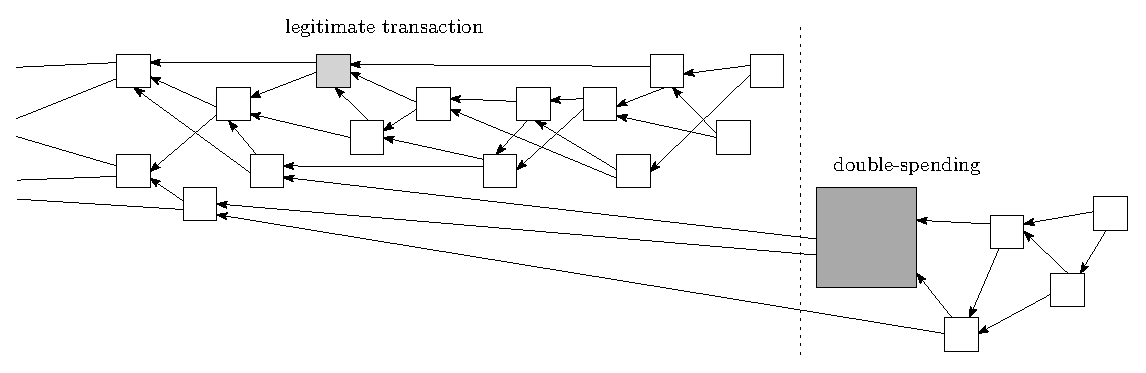
\includegraphics[width=\textwidth]{bigPoW} 
\caption{The ``large weight'' attack}
\label{f_bigPoW}
\end{figure}
The probability of this event is
\[
 \IP[W^{(n_0)}<t_0]=1-\exp(-t_0\mu 3^{-n_0})
  \approx 1-\exp(-t_0\mu w_1^{-1})
  \approx \frac{t_0\mu}{w_1}.
\]
This approximation is true in the case where 
$\frac{t_0\mu}{w_1}$ is small, which is 
a reasonable assumption. If this ``immediate'' attack
does not succeed, the attacker may continue to look for the nonce
that gives weight~$3^n$ for $n>n_0$, and hope that at the moment
they find it, the total weight of the legitimate branch is smaller
than~$3^n$. The probability of this event occurring is
\[
 \IP[\lambda w W^{(n)}<3^n]
=1-\exp\big(-\mu 3^{-n_0}\times (3^{n_0}/\lambda w)\big)
  = 1-\exp(- \mu/\lambda w)
  \approx \frac{\mu}{\lambda w}.
\]
That is, although $\frac{\mu}{\lambda w}$ should typically
be a small number, at each ``level'' $n$ the attack succeeds with a constant
probability. Therefore, it will a.s. succeed. 
%In fact,
The typical time until it succeeds 
is roughly $3^\frac{\lambda w}{\mu}$. Although this quantity
may be very large, the probability that the 
``first''\footnote{During the time~$t_0$.} attack succeeds 
is not negligible. 
%We thus arrive to the following conclusion:
Therefore, we need countermeasures. One such countermeasure 
would be limiting the own weight from above, or even setting 
it to a constant value. As mentioned in Section~\ref{s_cutsets}, the 
latter may not be the best solution because it does not offer 
enough protection from spam.
%For example,
%limit the own weight from above, or even set it to constant
%(as mentioned in Section~\ref{s_cutsets}, the latter
%may be not the best solution, since it does not 
%offer enough protection from spam).

\medskip

Now, let us discuss the situation
where the maximum own weight is capped at a value of~$1$,
 and estimate the probability that the attack succeeds.
 %(the general case can be treated in the same
%way, simply by rescaling)

Assume that a given transaction gained
 cumulative weight~$w_0$ in~$t_0$ time units after the moment
when it was issued, and
%Assume also 
that the adaptation period for 
that transaction is over. In this situation, the transaction's
 cumulative weight
increases linearly with speed~$\lambda $. Now, 
imagine that the attacker wants to double-spend on this transaction.
To do so, the attacker secretly prepares the double-spending transaction,
 and starts generating \emph{nonsense} transactions 
that approve the double-spending transaction at the 
time\footnote{Or even before; we discuss this case later.}
 when the \emph{original} transaction was issued to the merchant.
%he/she secretly prepares the double-spending transaction, 
%and starts generating other transactions
%that approve the double-spending one. 
If 
%at some moment
%(after the merchant decides to accept the legitimate
%transaction) 
the attacker's subtangle outpaces the legitimate
subtangle at some moment after the merchant decides to accept 
the legitimate transaction, then the double-spending attack would be successful.
If that does not happen, then
the double-spending transaction 
would not be approved by others 
because the legitimate transaction would acquire more cumulative 
weight and essentially all new tips would indirectly 
approve it. The double-spending transaction would be orphaned in 
this scenario.
% and so it will be orphaned.

As before, let~$\mu$ stand for the computing power of the attacker.
%(i.e., the speed of transactions' generation). 
We also make a simplifying assumption that the 
transactions propagate instantly.
Let $G_1,G_2, G_3,\ldots$ denote i.i.d.\ exponential 
random variables with parameter~$\mu$\footnote{With expected
 value~$1/\mu$.}, and define
$V_k=\mu G_k$, $k\geq 1$. It follows that
$V_1,V_2, V_3,\ldots$ are i.i.d.\ exponential 
random variables with parameter~$1$. 

Suppose that at time~$t_0$ the merchant decides to accept
the transaction with cumulative weight~$w_0$.
%(recall that it has cumulative weight~$w_0$
%at that time).
Let us estimate the probability that the attacker
successfully double-spends. Let $M(\theta)=(1-\theta)^{-1}$
be the moment generating function of the exponential
distribution with parameter~$1$ (Section~7.7
of~\cite{Ross}). 
It is known\footnote{This is a consequence of the so-called
Large Deviation Principle.
See the general book~\cite{DZ}, and
 Proposition~5.2 in Section~8.5 of~\cite{Ross}
for a simple and instructive derivation of the 
upper bound, and Section~1.9 of~\cite{Dur} for the 
(not so simple) derivation of the lower bound.} that for~$\alpha\in (0,1)$ it holds that
\begin{equation}
\label{Chernoff}
 \IP\Big[\sum_{k=1}^n V_k \leq \alpha n\Big] \approx
   \exp\big(-n\phi(\alpha)\big), 
\end{equation}
where $\phi(\alpha)=-\ln \alpha + \alpha -1$ is the Legendre
transform of $\ln M(-\theta)$. 
%Observe that, 
As a general fact,
it holds that $\phi(\alpha)>0$ for~$\alpha\in (0,1)$. Recall
that the expectation of an exponential random variable 
with parameter~$1$ also equals~$1$.

Assume that $\frac{\mu t_0}{w_0}<1$, otherwise the probability
that the attacker's subtangle
eventually outpaces the legitimate subtangle would be close to~$1$.
Now, to outweigh~$w_0$ at time~$t_0$, the attacker needs
to be able to issue at least $w_0$ 
%(for simplicity, we drop the integer parts) 
transactions with maximum own weight~$m$
during time~$t_0$. 
Therefore, using~\eqref{Chernoff}, we find
 the probability that the double-spending transaction
has more cumulative weight at time~$t_0$
is roughly
\begin{align}
 \IP\Big[\sum_{k=1}^{w_0/m} G_k  < t_0\Big]
 & = \IP\Big[\sum_{k=1}^{w_0} V_k  < \mu t_0\Big]
\nonumber\\
& = \IP\Big[\sum_{k=1}^{w_0} V_k  < w_0
\times\frac{\mu t_0}{w_0}\Big]
\nonumber\\
 & \approx \exp\big(-w_0
\phi\big(\textstyle\frac{\mu t_0}{w_0}\big)\big).
\label{double_t0}
\end{align}
For the above probability to be small,
$\frac{w_0}{m}$ needs to be large 
and~$\phi\big(\textstyle\frac{\mu t_0}{w_0}\big)$
cannot be very small. 

Note that, at time~$t\geq t_0$, the cumulative weight
of the legitimate transaction is roughly~$w_0+\lambda (t-t_0)$
because we assumed that the adaptation period is over,
so the cumulative weight grows with speed~$\lambda$.
Analogous to~\eqref{double_t0}, 
one finds the probability that the double-spending transaction
has more cumulative weight at time~$t\geq t_0$ is roughly
\begin{equation}
\label{double_t}
 \exp\big(-(w_0+\lambda (t-t_0))
\phi\big(\textstyle\frac{\mu t}{w_0+\lambda (t-t_0)}\big)\big).
\end{equation}
Then, it must be true that we have $\frac{\mu t_0}{w_0}\geq 
\frac{\mu}{\lambda}$ since the cumulative weight grows with 
speed less than~$\lambda $ during the adaptation period. 
It can be shown that the probability 
of achieving a successful double spend is of order
\begin{equation}
\label{double_ever}
 \exp\big(-w_0\phi\big(\max(\textstyle\frac{\mu t_0}{w_0},
\frac{\mu}{\lambda})\big)\big).
\end{equation}
For example, let $\mu=2$, $\lambda=3$
so that the attacker's power is only a bit less than
that of the rest of the network. Assume that the 
transaction has a cumulative weight of~$32$ by time~$12$.
Then, $\max(\frac{\mu t_0}{w_0},\frac{\mu}{\lambda}) = \frac{3}{4}$,
$\phi\big(\frac{3}{4}\big)\approx 0.03768$,
and~\eqref{double_ever} then gives the upper bound 
approximately $0.29$. If one assumes that
$\mu=1$ and keeps all other parameters intact, then
$\max(\frac{\mu t_0}{w_0},\frac{\mu}{\lambda}) = \frac{3}{8}$,
$\phi\big(\frac{3}{8}\big)\approx 0.3558$,
and~\eqref{double_ever} gives approximately $0.00001135$,
quite a drastic change.


 From the above discussion it is important to recognize that 
 the inequality $\lambda > \mu$ should be true for the 
 system to be secure. 
% for the system to be secure, it should be true that 
% $\lambda > \mu$ 
% (otherwise, the estimate~\eqref{double_ever} would be useless); i.e.,
In other words, the input flow of ``honest''
transactions should be large compared to the 
attacker's computational power. Otherwise, 
the estimate~\eqref{double_ever} would be useless. 
This indicates the need
for additional security measures, such as checkpoints,
during the early days of a tangle-based system.


%Also, as for the strategies for deciding which 
%one of two conflicting transactions is valid,
% one has to be careful when relying only on the cumulative 
When choosing a strategy for deciding which one of 
two conflicting transactions is valid, one has to be careful 
when using cumulative weight as a decision metric. 
This is due to the fact that cumulative weight can be subject
 to an attack similar
to the one described
in Section~\ref{s_parasite}, namely the attacker may prepare 
a double-spending transaction well in advance, build a 
secret subtangle referencing it, and then broadcast 
that subtangle after the merchant accepts the legitimate 
transaction.  
% Rather
A better method for deciding 
between two conflicting transactions might be the one
described in the next section: run the tip selection algorithm
and see which of the two transactions is indirectly
approved by the selected tip.

\subsection{A parasite chain attack and a new tip 
selection algorithm}
\label{s_parasite}
Consider the following attack (Figure~\ref{f_tip_Markov}):
an attacker secretly builds a subtangle that occasionally 
references the main tangle to gain a higher score. 
Note that the score of honest tips is roughly the sum 
of all own weights in the main tangle, while the score
of the attacker's tips also contains the sum of all own weights in the
parasite chain.
Since network latency is not an issue for an attacker
 who builds a subtangle 
alone\footnote{This is due to the fact that an attacker can always
approve their own transactions without relying on any
information from the rest of the network.},
they might be able to give more height
to the parasite tips if they use a computer 
that is sufficiently strong. Moreover, the attacker can artificially 
increase their tip count at the moment of the attack by 
broadcasting many new transactions that approve 
transactions that they issued earlier on the parasite chain
%Finally, the number of attacker's tips 
%can be artificially increased at the moment of the attack
%(by issuing a lot of transactions that all approve
%\emph{the same} attacker's transactions,
%see 
(Figure~\ref{f_tip_Markov}).
This will give the attacker an advantage in the case where 
the honest nodes use some selection strategy 
that involves a simple choice between available tips.

To defend against this attack style,
we are going to use the fact that the main tangle is supposed
to have more active hashing power than the attacker. Therefore, the 
main tangle is able to produce larger increases in cumulative weight 
for more transactions than the attacker.  
%manages to give more cumulative weight to more transactions than the attacker.
The idea is to use a MCMC algorithm
to select the two tips to reference. 

Let $\HH_x$ be the current cumulative weight of a site.
 %(i.e., a transaction represented on the tangle graph). 
 Recall that we assumed all 
own weights are equal to~$1$. Therefore, the cumulative weight of a tip
is always~$1$, and the cumulative weight of other sites is at least~$2$.

The idea is to place some particles, a.k.a.\ random walkers,
on sites of the tangle and let them walk towards the tips
in a random\footnote{There is not a ``canonical'' source of randomness.
The nodes just use their own (pseudo)random number generators
to simulate the random walks.} way. The tips ``chosen'' by the walks
are then the candidates for approval.
The algorithm is described in the following way:
\begin{enumerate}
 \item Consider all sites on the interval $[W,2W]$, where 
 $W$ is reasonably large\footnote{The idea is to place the particle ``deep'' into
the tangle so that it will not arrive at a tip straight away. However, the 
particle should not be placed ``too deep'' because it needs to find a tip
 in a reasonable time. Also, the interval $[W,2W]$ is arbitrary. 
One could chose $[W,5W]$, etc.
There are also other ways to select the walkers' starting points.
 For example, a node can simply
take a random transaction received between $t_0$ and
$2t_0$ time units in the past, where~$t_0$ is some fixed time point.}.
% transactions with cumulative weight
% between $W$ and (say) $2W$ (where~$W$ 
%is reasonably large, to be chosen

 \item Independently place $N$ particles on sites in that
  interval\footnote{This choice
is largely arbitrary. We use several particles instead of just two
for additional security. The idea is that if a particle
were to accidentally jump to the attacker's chain, which is supposed
to be long, then it would spend a lot of time there 
and other tips will be chosen first.}.
  % there ($N$ is not so big, say, $10$ or so
 
 \item Let these particles perform independent
 discrete-time random
 walks ``towards the tips'', meaning that a transition
  from~$x$ to~$y$
is possible if and only if~$y$ approves~$x$
 \item The two random walkers that reach the tip set first will
sit on the two tips that will be approved.
However, it may be wise to modify this rule in the 
following way: first discard those random walkers that 
reached the tips \emph{too fast} because they may have ended on one
of the ``lazy tips''.
 \item The transition probabilities
 of the walkers are defined in the following
 way: if~$y$ approves~$x$ ($y\rightsquigarrow x$), 
then the transition probability~$P_{xy}$
 is proportional to $\exp\big(-\alpha(\HH_x-\HH_y)\big)$,
that is
 \begin{equation}
  \label{trans_probs}
   P_{xy} = \exp\big(-\alpha(\HH_x-\HH_y)\big)
\Big(\sum_{z: z \rightsquigarrow x}
 \exp\big(-\alpha(\HH_x-\HH_z)\big)\Big)^{-1},
 \end{equation}
where $\alpha>0$ is a parameter to be chosen\footnote{One can start 
with $\alpha=1$.}.
\end{enumerate}
Note that this algorithm is ``local'', meaning one does not need
 to traverse the tangle back to the genesis to perform relevant calculations.
In particular, 
observe that one does not need to calculate the cumulative
weights for the whole tangle. At most one needs to calculate the 
cumulative weights 
for the sites that indirectly approve the starting point
of the walker.


\begin{figure}
 \centering 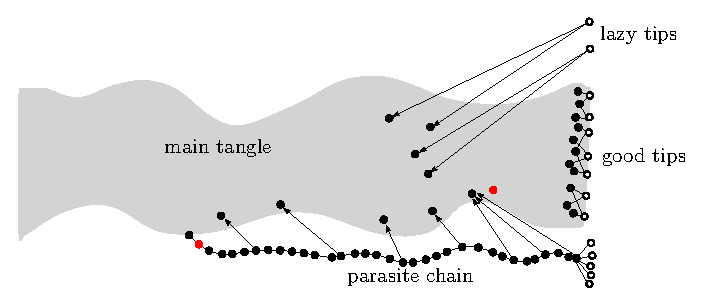
\includegraphics[width=0.81\textwidth]{tip_Markov} 
\caption{Visual representation of the tip selection algorithm for 
honest tips, as well as the parasite chain. The two red circles 
indicate an attempted double-spend by an attacker.
%On the tip selection algorithm. The two red circles indicate
%an attempted double-spend.
}
\label{f_tip_Markov}
\end{figure}

To check that the algorithm works as intended, first consider the ``lazy
tips''. These tips intentionally approve some old transactions
to avoid doing verification work (Figure~\ref{f_tip_Markov}).
Even if the particle 
is on a site approved by a lazy tip, it is not probable that the lazy
tip would be selected because the difference between cumulative
 weights would be very large and~$P_{xy}$ would be small.
 %, look at~\eqref{trans_probs}.

Next, consider this alternate attack style: the attacker secretly builds
a chain 
%(a ``parasite chain'')
 containing a transaction that empties their account balance to 
another account under their control, indicated as the leftmost red
circle in Figure~\ref{f_tip_Markov}. Then, the attacker
issues a transaction on the main tangle, represented by the rightmost red circle,
and waits for the merchant to accept it. The parasite chain occasionally
references the main tangle. However, the cumulative weight is not very 
large in the parasite chain. It should be noted that the parasite chain cannot 
reference the main tangle after the merchant's transaction. Furthermore, 
% and so its sites have
%good height/score (even better than those of the main tangle),
%although the cumulative weight is not so big in that chain. 
%Note also that it cannot reference the main tangle after 
%the merchant's transaction. Also, 
the attacker might try to artificially
inflate the number of tips in their parasite chain 
at the moment of the attack (Figure~\ref{f_tip_Markov}).
%as shown on the picture. 
The attacker's idea is to make the nodes issuing new transactions 
reference the parasite chain so that the honest branch of the tangle will
be orphaned.

It is easy to see why the MCMC selection algorithm
 will not select one of the attacker's tips with high probability.
%Basically, the 
The reasoning is identical to the lazy tip scenario:
%the same as why the algorithm does not 
%select the lazy tips:
 the sites on the parasite chain will
have a cumulative weight that is much smaller 
than the sites that they reference on the main tangle.
 Therefore, it is not probable that the random
walker will ever jump to the parasite chain unless it begins there,
and this event is not very probable either because the main tangle contains
more sites. 

As an additional protecting measure, we can 
first ran a random walk with a large~$\alpha$ (so that it is 
in fact ``almost deterministic'') to choose a 
 ``model tip''; then, use random walks with small~$\alpha$
for actual tip selection, but verify if the (indirectly)
referenced transactions are consistent with the model tip.

Observe also that,
for a random walk that \emph{always} moves towards the tips 
it is very simple and rapid to calculate the exit probability distribution using a straightforward recursion; this is something
that we \emph{do not} want the nodes to do. 
However, it is possible to modify our approach in the following
way: on each step, the random walk may
 backtrack (i.e., go 1 step away from the tips) 
with probability (say) $\frac{1}{3}$ 
(and divide the remaining $\frac{2}{3}$ as before). 
The walk will reach the tips very queckly anyway 
(because it has a drift towards the tips), 
but it will not be so easy to calculate the exit measure. 
% It is good that it's not easily calculable -- 
% the "selfish" nodes won't have easy time.

Let us comment on why 
 the nodes would follow this algorithm.
Recall from Section~\ref{s_general} that
it is reasonable to assume that at least a ``good'' proportion
of the nodes will follow the \emph{reference} algorithm.
Also, because of computational and network delays, the 
tip selection algorithm would rather work with a past snapshot
of the tangle with respect to the moment when a transaction
is issued. \emph{It may be a good idea to intentionally
move this snapshot to a time point further in the past\footnote{First
the random walker finds a former tip with respect to that snapshot,
and then it continues to walk towards the ``actual'' tips
on the current tangle.}} in the reference algorithm 
for the reasons that we explain in the sequel.
Imagine a ``selfish'' node that just wants to maximize 
the chances of their transaction being approved quickly.
The MCMC algorithm of this section, which is adopted by a
 considerable proportion of nodes, 
defines a probability
distribution on the set of tips. 
It is clear that a natural first choice for a selfish node would be
to choose the tips where the maximum of that distribution 
is attained. However, if many other nodes also behave
in a selfish way 
%(which is quite reasonable to assume as well)
 and use the same strategy, which is a reasonable assumption, 
 then they all 
will lose. \emph{Many} new transactions will approve 
the same two tips at roughly the same time, therefore
generating too much competition between them for subsequent approval.
It should also be clear that nodes will not immediately ``feel'' the cumulative 
weight increase caused by this mass approval of the same two tips since 
the nodes are using a past snapshot.
%Since the nodes use a past snapshot, they will not yet ``feel''
%the cumulative weight increase caused by this mass approval
%of the two tips.
 For this reason, even a selfish node would have 
to use some random tip approval algorithm\footnote{as noticed
before, for a backtracking walk there 
seem to be no easy way to discover which tips are 
 better (that is, more likely to be selected
by ``honest'' nodes) other than running the MCMC many times.
However, running MCRW many times requires time and other
resources; after one spends some time on it, 
the state of the tangle will already change, 
so one would possibly even have to start anew.
This explains why nodes do not have reasons
to abandon the MCMC tips selection strategy in favor
of something else, at least if they assume that a 
considerable proportion of the other nodes follow
the default tips selection strategy.}
 with a 
probability distribution for tip selection that is close to
% the selected tips should
%be, in some sense, ``not far away'' from
 the default probability distribution produced
by the reference tip selection algorithm.
We do not claim that this ``aggregated'' probability
distribution
would be equal to the default probability distribution in the presence of selfish nodes. 
However, the above argument shows that it should be close to it.
This means that the probability of many nodes attempting 
to verify the same ``bad'' tips would remain small. 
% selecting ``bad'' tips would remain small. 
In any case, 
%(differently from Bitcoin), 
there is not a large incentive for the nodes to be selfish 
because possible gains only amount to a slight decrease 
in confirmation time. This is inherently different from other 
decentralized constructs, such as Bitcoin. The important 
fact is that nodes do not have reasons to abandon the
 MCMC tip selection algorithm.


We would like to mention that the definition of transition 
probabilities, as given in~\eqref{trans_probs}, has not been 
set in stone.
% Also, it is not set in stone that the transition probabilities
%should necessarily be defined as in~\eqref{trans_probs}.
Instead of the exponent, one can use a different function 
that decreases rapidly, such~$f(s)=s^{-3}$. 
There is also freedom for choosing~$W$ and~$N$ as well.
At this point in time, it is unclear if there are any theoretical 
arguments that show exactly in which way these parameters 
should be chosen. In sum, we feel that the main contribution 
of this section is the idea of using MCMC for tip selection.
%In fact, the author's feeling is that the main contribution
%of this section is the very idea of using MCMC for tip selection;
%it is unclear if there is any ``theoretical''
%argument that shows exactly in which way these parameters
%must be chosen.

\subsection{Splitting attack}
\label{s_splitting}
Aviv Zohar suggested the following attack scheme against the 
proposed MCMC algorithm.
In the high-load regime, 
an attacker can try to split the tangle into two branches 
 and maintain the balance between them.
This would allow both branches to continue to grow.  
The attacker must place at least 
two conflicting transactions at the beginning of the split to prevent an honest node from effectively joining the branches 
by referencing them both simultaneously.
% Thereby split the power of the entire network. The network itself 
% work (because of the use of MCMC) almost equally to both sectors 
% and an attacker would only spend a little to balance. 
% In other words, weak inhibitor valid decision at will and splits 
% the computing power of the network to monitor contradictory versions. 
% It can also incorporate double spend parallel attacks.
Then, the attacker hopes that roughly half of the network would
contribute to each branch so that they 
would be able to ``compensate'' for random fluctuations,
even with a relatively small amount of personal computing power. 
If this technique works, the attacker would be able to spend the same
funds on the two branches.

To defend against such an attack, one needs to use a
``sharp-threshold'' rule 
%(like ``select the longest chain'' in Bitcoin) 
that makes it too hard to maintain the balance
between the two branches. An example of such a rule is 
selecting the longest chain on the Bitcoin network. Let us 
translate this concept to the tangle when it is undergoing a 
splitting attack. Assume that
the first branch has total weight 537, and the second branch 
has total weight 528. If an honest
node selects the first branch with probability very close to~$1/2$,
then the attacker would probably be able to maintain the
balance between the branches. However, if an honest
node selects the first branch with probability
much larger than $1/2$, then the attacker would probably
be unable to maintain the
balance. The inability to maintain balance between the two branches in 
the latter case is due to the fact that after an inevitable random fluctuation,
the network will quickly choose one of the branches and abandon the other. 
In order to make the MCMC algorithm behave this way,
one has to choose a very rapidly decaying function~$f$,
and initiate the random walk at a node with
 large depth so that it is highly probable
that the walk starts before the branch bifurcation.
In this case, the random walk would choose the ``heavier''
branch with high probability, even if the difference in
 cumulative weight between the competing branches is small. 

It is worth noting that the attacker's task is very 
difficult because of network synchronization
issues: they may not be aware of a large number 
of recently issued transactions\footnote{The ``real''
cumulative weights may be quite different from 
what they believe.}. Another effective 
method for defending against a 
splitting attack would be for a sufficiently
powerful entity to instantaneously publish a large number
 of transactions on one branch, thus rapidly changing the power balance
and making it difficult for the attacker to deal with this change. 
If the attacker manages to maintain
the split, the most recent transactions will only have around $50$\%
 confirmation confidence (Section~\ref{s_general}), and the branches 
will not grow. In this scenario, the ``honest'' nodes may decide to start 
selectively giving their approval to the transactions that occurred before 
the bifurcation, bypassing the opportunity to approve the conflicting 
transactions on the split branches.
%only the pre-split transactions then (and, in particular,
%not approve neither of the two conflicting transactions).

One may consider other versions of the 
tip selection algorithm. For example, if a node sees
 two big subtangles, 
then it chooses the one with a larger sum of own weights 
before performing the MCMC tip selection algorithm outlined above.
%and then does the tip selection only there using the 
%above MCMC algorithm. 

The following idea may be worth considering for future implementations. 
One could make the transition probabilities defined 
in~\eqref{trans_probs} depend 
on both $\HH_x-\HH_y$ and $\HH_x$ in such a 
way that the next step of the Markov chain is almost deterministic
when the walker is deep in the tangle, yet becomes more 
random when the walker is close to tips. This will help avoid entering the 
weaker branch while assuring sufficient randomness when choosing the 
two tips to approve.
% (so that there is enough randomness in the choice
%of the two transactions to approve). 



\paragraph{Conclusions:}
\begin{enumerate}
 \item We considered attack strategies for when an 
attacker tries to double-spend by ``outpacing'' the system.
 \item The ``large weight'' attack means that, in order to 
double-spend, the attacker tries to give a very large weight
to the double-spending transaction so that it would 
outweigh the legitimate subtangle. This strategy would be 
a menace to the network in the case where the allowed own weight is
unbounded. As a solution, we may limit the own weight
of a transaction from above, 
or set it to a constant value.
 \item In the situation where the maximal own weight
of a transaction is~$m$, the best attack strategy
is to generate transactions with own weight~$m$
that reference the double-spending transaction. 
When the input flow of ``honest''
transactions is large enough compared to the 
attacker's computational power, the probability
that the double-spending transaction
has a larger cumulative weight can be estimated
using the formula~\eqref{double_ever} (see also
examples below~\eqref{double_ever}).
 \item The attack method of building a ``parasite chain''
makes approval strategies based on height or score
obsolete since the attacker's sites will have higher values 
for these metrics when compared to the legitimate tangle. On the other hand,
the MCMC tip selection algorithm described in Section~\ref{s_parasite}
seems to provide protection against this kind of attack.
\item The MCMC tip selection algorithm also offers protection against 
the lazy nodes as a bonus.
%As a 
%bonus, it also offers protection against the ``lazy nodes'',
%i.e., those that just approve some old transactions to avoid 
%doing the calculations necessary for validating the tangle.
\end{enumerate}



\section{Resistance to quantum computations}
\label{s_quantum}
It is known that a sufficiently large
 quantum computer\footnote{Still a hypothetical construct as of today.}
  could be very efficient for handling problems
that rely on trial and error to find a solution. The process of finding a nonce
in order to generate a Bitcoin block is a good example 
of such a problem. As of today, one must 
check an average of $2^{68}$ nonces to find a suitable hash
that allows a new block to be generated. 
 It is known (see e.g.~\cite{BHT}) that a quantum computer would need 
$\Theta(\sqrt{N})$ operations to solve a problem that is analogous to 
the Bitcoin puzzle stated above. This same problem would need
~$\Theta(N)$ operations on a classical computer.
Therefore, a quantum computer would be 
around $\sqrt{2^{68}}=2^{34}\approx 17$ billion times
more efficient at mining the Bitcoin blockchain than a classical computer.
Also, it is worth noting that
 if a blockchain does not increase its difficulty in response 
to increased hashing power, there would be an 
increased rate of orphaned blocks.

For the same reason, a ``large weight'' attack would also be much more 
efficient on a quantum computer.
%described above would also be much more efficient on a quantum
%computer. 
However, capping the weight from above, as suggested
in Section~\ref{s_attacks}, would effectively prevent
a quantum computer attack as well. This is evident in iota because 
the number of nonces that one needs to check in order
to find a suitable hash for issuing a transaction is not 
unreasonably large. On average, it is around~$3^8$. 
The gain of efficiency for 
an ``ideal'' quantum computer would therefore
be of order $3^{4}=81$, which is already quite 
acceptable\footnote{Note that $\Theta(\sqrt{N})$
could easily mean $10\sqrt{N}$.}.
More importantly, the algorithm used in the iota implementation 
is structured such that the time to find a nonce is 
not much larger than the time needed for other tasks that 
are necessary to issue a transaction. The latter part is much
 more resistant against quantum computing, and therefore 
 gives the tangle much more protection against an adversary with a 
 quantum computer when compared to the (Bitcoin) blockchain.



\section*{Acknowledgements}
The author thanks  Bartosz Kusmierz, Cyril Gr\"unspan,
Olivia Saa, and
 Toru Kazama who pointed
out several errors in earlier drafts, and James Brogan
for his contributions towards making this paper more readable.



\begin{thebibliography}{9}
% \bibitem{iota_crypto}
% \textsc{Jinn Labs} (2015)  Iota whitepaper.
\bibitem{iota} Iota: a cryptocurrency for Internet-of-Things.
See \texttt{http://www.iotatoken.com/}, and
\texttt{https://bitcointalk.org/index.php?topic=1216479.0}

\bibitem{bitcoinj}  bitcoinj.  
Working with micropayment channels.\\
\texttt{https://bitcoinj.github.io/working-with-micropayments}

\bibitem{dag_generalized_blockchain}
\textsc{people on nxtforum.org}  (2014)
DAG, a generalized blockchain.
\texttt{https://nxtforum.org/proof-of-stake-algorithm/dag-a-generalized-blockchain/}  (registration at \texttt{nxtforum.org} required)

\bibitem{red_balloons}
\textsc{Moshe Babaioff, Shahar Dobzinski, Sigal Oren, Aviv Zohar} (2012)
On Bitcoin and red balloons.
\textit{Proc.\ 13th ACM Conf.\ Electronic Commerce}, 56--73. 


\bibitem{Dur} \textsc{Richard Durrett} (2004)
Probability -- Theory and Examples.
\textit{Duxbury advanced series.}


\bibitem{dagcoin} \textsc{Sergio Demian Lerner} (2015)
DagCoin: a cryptocurrency without blocks.
\texttt{https://bitslog.wordpress.com/2015/09/11/dagcoin/}

\bibitem{SZ} \textsc{Yonatan Sompolinsky, Aviv Zohar} (2013)
Accelerating Bitcoin's Transaction Processing.
Fast Money Grows on Trees, Not Chains.
\texttt{https://eprint.iacr.org/2013/881.pdf}

\bibitem{SZ_SPECTRE} 
 \textsc{Yonatan Sompolinsky, Yoad Lewenberg, Aviv Zohar} (2016)
SPECTRE:
Serialization of Proof-of-work Events: Confirming Transactions via
Recursive Elections.
%Yonatan Sompolinsky, Yoad Lewenberg, and Aviv Zohar
\texttt{https://eprint.iacr.org/2016/1159.pdf}

\bibitem{LSZ} \textsc{Yoad Lewenberg, Yonatan Sompolinsky, Aviv Zohar} 
(2015)
Inclusive Block Chain Protocols.\\
\texttt{http://www.cs.huji.ac.il/\textasciitilde{}avivz/pubs/15/inclusive\underline{\phantom{m}}btc.pdf}

\bibitem{lightning}
\textsc{Joseph Poon, Thaddeus Dryja} (2016)
The Bitcoin Lightning Network:
Scalable Off-Chain Instant Payments.\\
\texttt{https://lightning.network/lightning-network-paper.pdf}

\bibitem{Ross_m} \textsc{Sheldon M.\ Ross} (2012) 
\textit{Introduction to Probability Models.} 10th ed.

\bibitem{braids}
\textsc{David Vorick} (2015)
Getting rid of blocks.
\texttt{slides.com/davidvorick/braids}


\bibitem{DZ} 
\textsc{Amir Dembo, Ofer Zeitouni} (2010)
\textit{Large Deviations Techniques and Applications.}
Springer.

\bibitem{Ross} \textsc{Sheldon M. Ross} (2009) 
\textit{A First Course in Probability.} 8th ed.

\bibitem{BHT} \textsc{Gilles Brassard, Peter HØyer, Alain Tapp} (1998)
Quantum cryptanalysis of hash and claw-free functions.
\textit{Lecture Notes in Computer Science} \textbf{1380},
163--169.


\end{thebibliography}
\end{CJK}
\end{document}
